\documentclass{../../oss-apphys}
\usepackage{bm}

\begin{document}
\genheader

\gentitle{1 \& C}{MOMENTUM, IMPULSE, COLLISIONS, AND CENTER OF MASS}

\genmultidirections

\gengravity

\raggedcolumns
\begin{multicols}{2}

  \begin{enumerate}[leftmargin=18pt]

  \item A toy train car of mass \SI{3}{\kilo\gram} rolls to the left at
    \SI{2}{\metre\per\second} and collides with a \SI{4}{\kilo\gram} train
    car rolling to the right at \SI{1}{\metre\per\second}. The two cars stick
    together. The velocity of the cars after the collision is
    \begin{enumerate}[noitemsep,topsep=0pt,leftmargin=18pt,label=(\Alph*)]
    \item $2/7$ \si{\metre\per\second} to the left
    \item $2/7$ \si{\metre\per\second} to the right
    \item $4/7$ \si{\metre\per\second} to the left
    \item $4/7$ \si{\metre\per\second} to the right
    \item $9/7$ \si{\metre\per\second} to the right
    \end{enumerate}
    
  \item Two steel balls, one of mass m and the other of mass 2m, collide and
    rebound in a perfectly elastic collision. Which of the following is
    conserved in this elastic collision?
    \begin{enumerate}[noitemsep,topsep=0pt,leftmargin=18pt,label=(\Alph*)]
    \item velocity only
    \item momentum only
    \item momentum and kinetic energy only
    \item momentum, velocity, and kinetic energy
    \item kinetic energy only
    \end{enumerate}
%%Questions 153–154. A force acts on a 2.0 kg mass during a time interval as
%%shown in the graph.
%%153. The impulse given to the mass from t = 0 to t = 6 s is
%%(A) 4 N s
%%(B) 8 N s
%%(C) 12 N s
%%(D) 16 N s
%%(E) 24 N s
%%154. If the initial speed of the mass is 2 m/s at t = 0, what is its speed at the
%%end of 6 s?
%%(A) 4 m/s
%%(B) 6 m/s
%%(C) 8 m/s
%%(D) 10 m/s
%%(E) 16 m/s
    
%  \item A rubber ball of mass $m$ strikes a wall with a speed $v$ at an angle
%    $\theta$ below the normal line and rebounds from the wall at the same speed
%    and angle above the normal line as shown. The change in momentum
%    of the ball is
%    \begin{center}
%      \pic{.25}{ball-bounce-wall.png}
%    \end{center}
%    \begin{enumerate}[noitemsep,topsep=0pt,leftmargin=18pt,label=(\Alph*)]
%    \item $mv$
%    \item $2mv$
%    \item $mv\cos\theta$
%    \item $2mv\cos\theta$
%    \item  zero
%    \end{enumerate}
  
  \item Two blocks are connected by a compressed spring and rest on a
    frictionless surface. The blocks are released from rest and pushed apart
    by the compressed spring. If one mass is twice the mass of the other,
    which of the following is the same for both blocks?
    \begin{enumerate}[noitemsep,topsep=0pt,leftmargin=18pt,label=(\Alph*)]
    \item magnitude of momentum
    \item acceleration
    \item speed
    \item kinetic energy
    \item potential energy
    \end{enumerate}
    \columnbreak
    
  \item A \SI{1000}{\kilo\gram} railroad car is rolling without friction on a
    horizontal track at a speed of \SI{3.}{\metre\per\second}. Sand is poured
    into the open top of the car for a time of \SI{5.}{\second}. The speed of
    the car after \SI{5.}{\second} is \SI{1.}{\metre\per\second}. The mass of
    the sand added to the car at the end of \SI{5.}{\second} is
    \begin{center}
      \pic{.23}{railroad-car-sand.png}
    \end{center}
    \begin{enumerate}[noitemsep,topsep=0pt,leftmargin=18pt,label=(\Alph*)]
    \item\SI{500 }{\kilo\gram}
    \item\SI{1000}{\kilo\gram}
    \item\SI{2000}{\kilo\gram}
    \item\SI{3000}{\kilo\gram}
    \item\SI{3500}{\kilo\gram}
    \end{enumerate}
    
  \item Two billiard balls are rolling to the right on a table as shown. The
    \SI{.4}{\kilo\gram} ball is moving faster than the \SI{.2}{\kilo\gram}
    ball, so it catches up and strikes it from behind at a slight angle.
    Immediately after the collision, the $y$-component of the
    \SI{.4}{\kilo\gram} ball is \SI{2}{\metre\per\second} downward.
    The $y$-component of the velocity of the \SI{.2}{\kilo\gram} ball must be
    \begin{center}
      \pic{.23}{big-small-billiard-balls.png}
    \end{center}
    \begin{enumerate}[noitemsep,topsep=0pt,leftmargin=18pt,label=(\Alph*)]
    \item \SI{1}{\metre\per\second} upward
    \item \SI{2}{\metre\per\second} upward
    \item \SI{1}{\metre\per\second} downward
    \item \SI{2}{\metre\per\second} downward
    \item \SI{4}{\metre\per\second} upward
    \end{enumerate}
    \newpage
    
%%Questions 159–160. Two balls are on a horizontal billiard table. A 1.0 kg
%%billiard ball moves downward along the y-axis with a speed of 16 m/s toward
%%a 2.0 kg ball that is at rest. The balls collide at an angle, and move along the
%%lines shown. After the collision, the 1.0 kg ball moves at 9 m/s along the +x-
%%axis. The table below shows the x and y components of the momentum in kg
%%m/s of the two balls before and after the collision.
%%159. Which of the following statements is true?
%%(A) Momentum is conserved only in the x-direction in this collision.
%%(B) Momentum is conserved only in the y-direction in this collision.
%%(C) Momentum is conserved in both the x- and y-directions in this
%%collision
%%(D) The momentum of the 1.0 kg ball increases after the collision.
%%(E) The momentum of the 2.0 kg ball decreases after the collision.160. What is the speed of the 2.0 kg ball after the collision?
%%(A) 16.0 m/s
%%(B) 9.2 m/s
%%(C) 7.5 m/s
%%(D) 6.0 m/s
%%(E) 5.0 m/s
  \item A \SI{.3}{\kilo\gram} baseball at rest on a tee is struck by a bat. The
    ball leaves the at with a speed of \SI{20}{\metre\per\second} at an angle
    of \ang{45} above the horizontal. The magnitude of the impulse imparted to
    the baseball by the bat is most nearly
    \begin{enumerate}[noitemsep,topsep=0pt,leftmargin=18pt,label=(\Alph*)]
    \item\SI{2}{\newton\second}
    \item\SI{6}{\newton\second}
    \item\SI{12}{\newton\second}
    \item\SI{16}{\newton\second}
    \item\SI{20}{\newton\second}
    \end{enumerate}
    
  \item Two ice skaters, a large man and a small woman, are initially at rest
    and holding each other's hands. They push away horizontally. Afterward,
    which of the following statements is true?
    \begin{enumerate}[noitemsep,topsep=0pt,leftmargin=18pt,label=(\Alph*)]
    \item They have equal and opposite kinetic energies.
    \item The have equal and opposite momenta.
    \item The large man applies a greater force to the small woman.
    \item The small woman applies a greater force to the large man.
    \item They recoil with equal and opposite velocities.
    \end{enumerate}

  \item A small mass $m$ is moving with a speed $v$ toward a stationary mass
    $M$. The speed of the center of mass of the system is
    \begin{enumerate}[noitemsep,topsep=0pt,leftmargin=18pt,label=(\Alph*)]
    \item $\displaystyle\left(\frac{m}{m+M}\right)v$
    \item $\displaystyle\left(\frac{m+M}{m}\right)v$
    \item $\displaystyle\left(\frac{m}{M}\right)v$
    \item $\displaystyle\left(1+\frac{m}{M}\right)v$
    \item $\displaystyle\left(1+\frac{M}{3m}\right)v$
    \end{enumerate}

  \item A known net force $F$ acts on an unknown mass for a known time
    $\Delta t$. From this information, you could determine the
    \begin{enumerate}[noitemsep,topsep=0pt,leftmargin=18pt,label=(\Alph*)]
    \item change in kinetic energy of the object
    \item change in velocity of the object
    \item acceleration of the object
    \item mass of the object
    \item change in momentum of the object
    \end{enumerate}  
  \end{enumerate}
  \columnbreak
  
  \textbf{Questions \ref{explode1}--\ref{explode2}}. An object has a mass $4m$.
  The object explodes into three pieces of mass $m$, $m$, and $2m$. The two
  pieces of mass $m$ move off at right angles to each other with the same
  momentum $mv$, as shown.
  \begin{center}
    \pic{.25}{3-piece-bomb.png}
  \end{center}
  
  \begin{enumerate}[leftmargin=18pt,resume]
  \item The speed of mass $2m$ after the explosion is
    \label{explode1}
    \begin{enumerate}[noitemsep,topsep=0pt,leftmargin=18pt,label=(\Alph*)]
    \item $2v$
    \item $\displaystyle\sqrt{2}v$
    \item $\displaystyle\frac{\sqrt{2}}{2}v$
    \item $\displaystyle\frac{\sqrt{2}}{3}v$
    \item $\displaystyle\frac{\sqrt{3}}{2}v$
    \end{enumerate}
    
  \item The direction of velocity of mass $2m$ is
    \label{explode2}
    \begin{enumerate}[noitemsep,topsep=0pt,leftmargin=18pt,label=(\Alph*)]
    \item $\rightarrow$
    \item $\swarrow$
    \item $\downarrow$
    \item $\nearrow$
    \item $\uparrow$
    \end{enumerate}
  \end{enumerate}
  \columnbreak
  
%%165. A system consists of two blocks having masses of 2 kg and 1 kg. Theblocks are connected by a string of negligible mass and hung over a
%%light pulley, and then released from rest. When the speed of each block
%%is v, the momentum of the center of mass of the system is
%%(A) (2 kg + 1 kg)v
%%(B) (2 kg - 1 kg)v
%%(C) 1/3 (2 kg + 1 kg)v
%%(D) 1⁄2 (2 kg - 1 kg)v
%    %(E) (2 kg)v

  \textbf{Questions \ref{cm1}--\ref{cm2}}. A projectile is launched at an angle
  to the level ground as shown. At the top of the trajectory at point $P$, the
  projectile explodes into two pieces of mass $2m$ and $m$.
  \begin{center}
    \pic{.25}{exploding-projectile.png}
  \end{center}
  \begin{enumerate}[leftmargin=18pt,resume]
  \item Which of the following arrows best represents the direction of the
    velocity of the center of mass of the projectile at point $P$ after the
    explosion?
    \label{cm1}
    \begin{enumerate}[noitemsep,topsep=0pt,leftmargin=18pt,label=(\Alph*)]
    \item $\leftarrow$
    \item $\swarrow$
    \item $\searrow$
    \item $\rightarrow$
    \item $\nearrow$
    \end{enumerate}

  \item Which of the following statements is true of the center of mass of the
    projectile after the explosion?
    \label{cm2}
    \begin{enumerate}[noitemsep,topsep=0pt,leftmargin=18pt,label=(\Alph*)]
    \item The center of mass will continue on a parabolic path and land on
      the ground at the place where it would have landed had it not exploded.
    \item The center of mass will alter its parabolic path and land on the
      ground farther from where it would have landed had it not exploded.
    \item The center of mass will alter its parabolic path and land on the
      ground at a shorter distance than it would have landed had it not
      exploded.
    \item The center of mass will fall straight downward from the point of
      explosion.
    \item The center of mass will travel straight upward from the point of
      explosion.
    \end{enumerate}
    
%Questions 168–169. Two pieces of clay of equal mass m moving with equal
%speeds v o each traveling at an angle of 30° collide and stick together at the
%origin O as shown.
%168. Which of the following arrows represents the direction of the velocity
%of the combined mass after the collision?
%(A)
%(B)
%(C)
%(D)
%(E)
%169. The speed of the combined mass after the collision is
%(A) v o
%(B) 1⁄2 v o
%(C) 1⁄4 v o(D)
    %    %(E)
    
  \item A \SI{100}{\kilo\gram} cannon sits at rest with a \SI{1}{\kilo\gram}
    cannonball in the barrel. The cannonball is fired with a speed of
    \SI{50}{\metre\per\second} to the right, causing the cannon to recoil with
    a speed of \SI{.5}{\metre\per\second} to the left. The velocity of the
    center of mass of the cannon-cannonball system is
    \begin{enumerate}[noitemsep,topsep=0pt,leftmargin=18pt,label=(\Alph*)]
    \item zero
    \item\SI{5}{\metre\per\second} to the right
    \item\SI{5}{\metre\per\second} to the left
    \item\SI{50}{\metre\per\second} to the right
    \item\SI{50}{\metre\per\second} to the left
    \end{enumerate}
  \end{enumerate}
  \columnbreak
  
  \textbf{Questions \ref{3masses1}--\ref{3masses2}}. Three identical masses can
  slide freely on a horizontal surface as shown. The first mass moves with a
  speed of \SI{3.}{\metre\per\second} toward the second and third masses, which
  are initially at rest. The first and second mass collide elastically, and
  then the second and third masses collide inelastically.
  \begin{center}
    \pic{.4}{3-masses.png}
  \end{center}
  \begin{enumerate}[leftmargin=18pt,resume]
  \item The speed of the second mass after the collision is
    \label{3masses1}
    \begin{enumerate}[noitemsep,topsep=0pt,leftmargin=18pt,label=(\Alph*)]
    \item zero
    \item\SI{1.5}{\metre\per\second}
    \item\SI{3.}{\metre\per\second}
    \item\SI{6.}{\metre\per\second}
    \item\SI{9.}{\metre\per\second}
    \end{enumerate}

  \item The speed of the second and third masses after they collide
    inelastically is
    \label{3masses2}
    \begin{enumerate}[noitemsep,topsep=0pt,leftmargin=18pt,label=(\Alph*)]
    \item zero
    \item\SI{1.5}{\metre\per\second}
    \item\SI{3.0}{\metre\per\second}
    \item\SI{6.0}{\metre\per\second}
    \item\SI{9.0}{\metre\per\second}
    \end{enumerate}
  \end{enumerate}
  
%%173. The diagram in the figure shows the top view of two identical steel
%%balls on a horizontal table of negligible friction. The first ball moves
%%with a speed of 12 m/s and the second ball is initially at rest. After the
%%collision, the first ball moves with a speed of 8 m/s at an angle of 37°
%%to the vertical. Which of the following diagrams best represents the
%%approximate speed and direction of the second ball after the collision?
%%(A)(B)
%%(C)
%%(D)
%%(E)

      %175. A block of mass m is moving to the right with a speed v o on a
%%horizontal surface of negligible friction when it explodes. The
%%explosion causes the block to break into two pieces, each of which
%%moves in the horizontal direction. One piece of mass m/4 moves to the
%%left with a speed of 2v o . What is the velocity of the other piece?
%%(A)
%%(B)
%%(C)
%%(D)
%%(E)
%%2v o to the right
%%v o to the right
%%3⁄4 v o to the right
%%1⁄2 v o to the right
%%1⁄4 v o to the left
%%Questions 176–177. The graph shown indicates the force acting on a mass of
%%2 kg as a function of time.
%%176. For the time interval from t = 0 to t = 6 s, the change in momentum of
%%the 2 kg mass is
%%(A) 48 kg m/s
%%(B) 24 kg m/s
%%(C) 12 kg m/s
%%(D) -12 kg m/s
%%(E) zero
%%177. If the object starts from rest, the speed at the end of the time interval
%%from t = 0 to t = 3 s is
%%(A) zero(B)
%%(C)
%%(D)
%%(E)
%%12 m/s
%%18 m/s
%%24 m/s
%    %36 m/s
%    \columnbreak
    
%%179. The vector shown represents the initial momentum of a moving object.
%%The object collides with another object that is initially at rest. Which of
%%the diagrams below could represent the momenta of the colliding
%%objects after the collision?
%%(A)
%%(B)
%%(C)
%%(D)
%%(E)
  \textbf{Questions \ref{boy1}--\ref{boy2}}. A \SI{20}{\kilo\gram} boy runs at
  a speed of \SI{3.}{\metre\per\second} and jumps onto a \SI{40}{\kilo\gram}
  sled on frictionless ice that is initially at rest. The boy and the sled then
  move together for a short time.
  \begin{enumerate}[resume,leftmargin=18pt]
  \item The speed of the boy and sled after he jumps on it is
    \label{boy1}
    \begin{enumerate}[noitemsep,topsep=0pt,leftmargin=18pt,label=(\Alph*)]
    \item\SI{0.5}{\metre\per\second}
    \item\SI{0.8}{\metre\per\second}
    \item\SI{1.0}{\metre\per\second}
    \item\SI{1.5}{\metre\per\second}
    \item\SI{2.0}{\metre\per\second}
    \end{enumerate}
    
  \item While the boy and sled are moving, he jumps off the back of the sled in
    such a way the boy is at rest, and the sled continues to move forward.
    The speed of the sled after the boy jumps off is
    \label{boy2}
    \begin{enumerate}[noitemsep,topsep=0pt,leftmargin=18pt,label=(\Alph*)]
    \item\SI{1.5}{\metre\per\second}
    \item\SI{2.0}{\metre\per\second}
    \item\SI{3.0}{\metre\per\second}
    \item\SI{4.5}{\metre\per\second}
    \item\SI{6.0}{\metre\per\second}
    \end{enumerate}
  \end{enumerate}
%%Questions 182–183
%%A cart of mass m 1 is initially moving with a speed of 4.0 m/s on a track
%%toward a stationary cart of mass m 2 = 2 kg. After the collision, mass m 1
%%moves with a velocity of 1.5 m/s. The force vs. time graph is shown for the
%%time during the collision, with the collision beginning at t = 0.
%%182. The impulse each cart applies to the other is most nearly
%%(A) 40 N s
%%(B) 20 N s
%%(C) 10 N s
%%(D) 5 N s(E) 2 N s
%%183. The unknown mass m 1 is equal to
%%(A)
%%(B)
%%(C)
%%(D)
%%(E)
%%0.5 kg
%%1.5 kg
%%2.5 kg
%%4.0 kg
%%5.0 kg
%%184. A 1.0 kg block is released from rest from a height h at the top of a
%%fixed curved ramp of negligible friction. The block slides down the
%%ramp and collides with another block of mass 1.5 kg at rest at the
%%bottom of the ramp. The two blocks stick together and move with a
%%speed of 5 m/s. The height h from which the 1.0 kg block began is
%%(A) 0.8 m
%%(B) 1.2 m
%%(C) 1.8 m
%%(D) 2.8 m
%%(E) 7.8 m
%%185. A dart of mass m is fired into a wooden block of mass 4m that hangs
%%from a string. The dart and block then rise to a maximum height h. An
%%expression for the initial speed v o of the dart before striking the block is
%%(A)
%%(B)
%%(C)
  %%(D)

  \textbf{Questions \ref{ramps1}--\ref{ramps2}}. A small block of mass $m$
  slides on a horizontal frictionless surface toward a ramp of mass $3m$ which
  is also free to move on the surface. The small block slides up to a height
  $h$ on the ramp with no friction (Figure I), then they move together (Figure
  II), and the small block slides back down the ramp to the horizontal surface
  (Figure III). Both the block and the ramp continue to slide on the horizontal
  surface after they separate.
  \begin{center}
    \pic{.3}{Figs123.png}
  \end{center}
  \begin{enumerate}[resume,leftmargin=18pt]  
  \item Which of the following is true regarding the conservation laws
    throughout this process?
    \label{ramps1}
    \begin{enumerate}[noitemsep,topsep=0pt,leftmargin=18pt,label=(\Alph*)]
    \item Kinetic energy is conserved from Figure I to Figure II.
    \item Momentum is conserved from Figure I to Figure III.
    \item Kinetic energy is conserved from Figure II to Figure III.
    \item Potential energy is conserved from Figure I to Figure II.
    \item Potential energy is conserved from Figure II to Figure III.
    \end{enumerate}
    
  \item Which of the following is a true statement regarding Figure III?
    \label{ramps2}
    \begin{enumerate}[noitemsep,topsep=0pt,leftmargin=18pt,label=(\Alph*)]
    \item The small block is moving to the left and the ramp is moving to the
      right.
    \item The small block is moving to the right and the ramp is moving to the
      left.
    \item The small block is moving to the right and the ramp is moving to the
      right.
    \item The small block is moving to the left and the ramp is moving to the
      left.
    \item The small block and the large block are moving with the same velocity.
    \end{enumerate}
    \columnbreak
    
%%Questions 188–189. A rubber ball of mass m is released from rest from a
%%height h onto a fixed inclined plane angled at 45° to the horizontal. The ball
%%collides with the surface elastically.
%%188. Which of the following diagrams best indicates the direction of the
%%impulse vector J as it strikes the plane and the velocity vector v just
%%after it strikes the plane?
%%(A)
%%(B)
%%(C)
%%(D)
%%(E)
%%189. The speed of the ball just after striking the surface is(A)
%%(B)
%%(C)
%%(D)
%%(E)

  \item A \SI{1000}{\kilo\gram} (empty mass) railroad car is rolling without
    friction on a horizontal track at a speed of \SI{2.}{\metre\per\second}.
    Sand is poured into the open top of the car for the time interval from
    $t=0$ to $t=\SI{4.}{\second}$. The mass of the sand poured into the car as
    a function of time is $m(t)=60t^2$. The velocity of the car at a time of
    \SI{4.}{\second} is most nearly
    \begin{center}
      \pic{.25}{railroad-car-sand.png}
    \end{center}
    \begin{enumerate}[noitemsep,topsep=0pt,leftmargin=18pt,label=(\Alph*)]
    \item\SI{1}{\metre\per\second}
    \item\SI{2}{\metre\per\second}
    \item\SI{3}{\metre\per\second}
    \item\SI{4}{\metre\per\second}
    \item\SI{5}{\metre\per\second}
    \end{enumerate}
  \end{enumerate}
  
  \textbf{Questions \ref{remote1}--\ref{remote2}}. A remote controlled stunt
  car of mass \SI{800}{\kilo\gram} initially moving at
  \SI{10}{\metre\per\second} is crashed into a rail car of mass $m$ that is
  initially at rest. The cars stick together, and the speed $v$ of both cars
  after the collision is given by $\displaystyle v=\frac{6}{t+1}$.

  \begin{enumerate}[resume,leftmargin=18pt]
  \item By considering the fact that the crash occurs at time $t=0$, determine
    the mass $m$ of the rail car.
    \label{remote1}
    \begin{enumerate}[noitemsep,topsep=0pt,leftmargin=18pt,label=(\Alph*)]
    \item\SI{288}{\kilo\gram}
    \item\SI{445}{\kilo\gram}
    \item\SI{533}{\kilo\gram}
    \item\SI{698}{\kilo\gram}
    \item\SI{800}{\kilo\gram}
    \end{enumerate}
    
  \item The magnitude of the resisting force acting on the cars as a function of
    time after the collision is
    \label{remote2}
    \begin{enumerate}[noitemsep,topsep=0pt,leftmargin=18pt,label=(\Alph*)]
    \item $\displaystyle \frac{6m}{t+1}$
    \item $6m(t+1)$
    \item $6m(t+1)^2$
    \item $\displaystyle\frac{6m}{(t+1)^2}$
    \item $\displaystyle\frac{m(t+1)^2}{6}$
    \end{enumerate}
    
%%193. A force acts on a mass m according to the equation F = 12t 3 . If the
%%object starts from rest, the velocity of the object as a function of time is
%%(A) 36mt 3
%%(B)
%%(C)
%%(D)
%%(E)
%%194. A dart in a long blow gun starts from rest and gains a momentum
%%according to the equation p = 3t 3 + 2t while moving through the barrel
%%of the gun. The net force acting on the dart after 0.2 s is
%%(A) 1.2 N
%%(B) 2.4 N
%%(C) 6.0 N(D) 12.2 N
%%(E) 16.1 N
%%195. A variable force acts on a mass causing it to accelerate. If a graph of
%%this force vs. time is plotted, the change in momentum of the mass can
%%be determined by finding the
%%(A) slope of the graph
%%(B) area under the graph
%%(C) y-intercept of the graph
%%(D) x-intercept of the graph
%%(E) change in slope of the graph
%%196. A moving object is changing its momentum during a time interval. If a
%%graph of momentum vs. time is plotted, the net force acting on the mass
%%at any time can be determined by finding the
%%(A) slope of line tangent to the graph at that time
%%(B) area under the graph
%%(C) y-intercept of the graph
%%(D) x-intercept of the graph
%%(E) change in slope of the graph from beginning to end
    \columnbreak
    
  \item Two masses moving along the coordinates axes as shown collide at the
    origin and stick to each other. What is the angle $\theta$ that the final
    velocity that makes with the $x$-axis?
    \begin{center}
      \begin{tikzpicture}[scale=.7]
        \draw(-4,0)--(4,0);
        \draw(0,-3)--(0,3);
        \draw[thick,->](-2.5,0)--(-1,0)node[midway,below]{\tiny$\mb{v}_1$};
        \draw[thick,->](0,-2)--(0,-1)  node[midway,right]{\tiny$\mb{v}_2$};
        \draw[thick,->](0,0)--(1.3,1.3)node[pos=1,right]{\tiny$\mb{v}_f$};
        \draw[fill=gray](-2.5,0) circle(.2) node[above]{\tiny$m_1$};
        \draw[fill=gray](0,-2) circle(.2) node[right]{\tiny$m_2$};
        \draw[<->] (.75,0) arc(0:45:.75) node[pos=.6,right]{\tiny$\theta$};
      \end{tikzpicture}
    \end{center}
    \begin{enumerate}[noitemsep,topsep=0pt,leftmargin=18pt,label=(\Alph*)]
    \item $\tan^{-1}(v_2/v_1)$
    \item $\tan^{-1}[m_1v_1/(m_1+m_2)]$
    \item $\tan^{-1}(m_1v_2/m_2v_1)$
    \item $\tan^{-1}(m_2v_2^2/m_1v_1^1)$
    \item $\tan^{-1}(m_2v_2/m_1v_1)$
    \end{enumerate}
    
  \item A mass traveling in the $+x$ direction collides with a mass at rest.
    Which of the following statements is true?
    \begin{enumerate}[noitemsep,topsep=0pt,leftmargin=18pt,label=(\Alph*)]
    \item After the collision, the two masses will move with parallel velocities
    \item After the collision, the masses will move with anti-parallel velocities
    \item After the collision, the masses will both move along the x-axis
    \item After the collision, the $y$-components of the velocities of the two
      particles will sum to zero.
    \item None of the above
    \end{enumerate}
    \columnbreak
    
  \item A mass $m_1$ initially moving at speed $v_0$ collides with and sticks
    to a spring attached to a second, initially stationary mass $m_2$. The two
    masses continue to move to the right on a frictionless surface as the
    length of the spring oscillates. At the instant that the spring is
    maximally extended, the velocity of the first mass is
    \begin{center}
      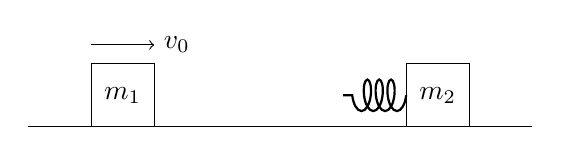
\begin{tikzpicture}[scale=.8]
        \draw[->](1,1.3)--(2,1.3) node[pos=1,right]{$v_0$};
        \draw(0,0)--(8,0);
        \draw(1,0) rectangle (2,1) node[midway]{$m_1$};
        \draw(6,0) rectangle (7,1) node[midway]{$m_2$};
        \draw[thick,
          decoration={aspect=.4,segment length=1.5mm, amplitude=2mm,coil},
          decorate] (6,.5)--(5,.5);
      \end{tikzpicture}
    \end{center}
    \begin{enumerate}[noitemsep,topsep=0pt,leftmargin=18pt,label=(\Alph*)]
    \item $v_0$
    \item $m_1^2v_0/(m_1+m_2)^2$
    \item $m_2v_0/m_1$
    \item $m_1v_0/m_2$
    \item $m_1v_0/(m_1+m_2)$
    \end{enumerate}

%  \item Two blocks of mass $m_A$ and $m_B$ are connected by a string that
%    passes over a light pulley. The mass of $A$ is larger than the mass of $B$.
%    The speed of mass $A$ just before reaching the floor is:
%    \begin{center}
%      \pic{.2}{pulley-a-b.png}
%    \end{center}
%    \begin{enumerate}[noitemsep,topsep=0pt,leftmargin=18pt,label=(\Alph*)]
%    \item $\displaystyle\sqrt{2\frac{m_A-m_B}{m_A+m_B}gD}$
%    \item $\displaystyle\sqrt{2\frac{m_A+m_B}{m_A-m_B}gD}$
%    \item $\displaystyle\sqrt{\frac{m_A}{m_A+m_B}gD}$
%    \item $\displaystyle\sqrt{\frac{m_B}{m_A+m_B}gD}$
%    \item $\displaystyle\sqrt{\frac{m_A}{m_B}gD}$
%    \end{enumerate}
  \end{enumerate}
\end{multicols}
\newpage


\genfreetitle{1 \& C}{MOMENTUM, IMPULSE, COLLISIONS, AND CENTER OF MASS}{5}

\genfreedirections{10}

\begin{enumerate}[leftmargin=15pt]
\item A projectile is fired from the edge of a cliff \SI{100}{\metre} high with
  an initial speed of \SI{60}{\metre\per\second} at an angle of elevation of
  \ang{45}.
  \begin{enumerate}[noitemsep]
  \item Write equation for $x(t)$, $y(t)$, $v_x$ and $v_y$. Choose the origin of
    your coordinate system at the particle's original location.
    \vspace{1.25in}
  \item Calculate the location and velocity of the particle at time
    $t=\SI{5}{s}$.
    \vspace{1.25in}
  \end{enumerate}
  Suppose the projectile experiences an internal explosion at time $t=\SI{4}{s}$
  with an internal force purely in the $y$-direction, causing it to break into
  a \SI{2}{\kg} and a \SI{1}{\kg} fragment.
  \begin{enumerate}[noitemsep,resume]
  \item If the \SI{2}{\kg} fragment is \SI{77}{m} above the height of the
    cliff at $t=\SI{5}{s}$, what is the $y$-coordinate of the position of the
    \SI{1}{\kg} piece?
    \vspace{1.25in}
  \item If the speed of the \SI{2}{kg} fragment is \SI{46}{m/s} and the
    fragment is falling at $t=\SI{5}{s}$, what is the $y$-component of the
    velocity of the \SI{1}{kg} fragment?
  \end{enumerate}
  \newpage
  
\item The Ballistic Pendulum. To determine the muzzle speed of a gun, a bullet
  is shot into a mass $M$ from a string as shown below, causing $M$ to swing
  upward through a maximum angle of $\theta$.
  \begin{center}
    \pic{.4}{ballastic.png}
  \end{center}
  \begin{enumerate}[noitemsep]
  \item What is the speed of $M$ the instant after the bullet lodges in it?
    \vspace{1.25in}
  \item What is the speed of the bullet before it hits $M$?
    \vspace{1.25in}
  \item What is the tension in the string at the highest point of the pendulum's
    swing (when the string makes an angle of $\theta$ with the vertical as
    shown)?
  \end{enumerate}
  \newpage
\item Two masses are connected by a spring (spring constant $k$) resting on a
  frictionless horizontal surface as shown. The right mass is initially in
  contact with a wall. A brief blow to the left block leaves it with an initial
  velocity $v_0$ to the right.
  \begin{enumerate}[leftmargin=18pt]
  \item What is the maximum compression of the spring as the left block moves
    to the right?
    \vspace{1in}
  \end{enumerate}
  After the spring is maximally compressed, it eventually moves to the left,
  away from wall. As it moves away from the wall, it continues oscillating.
  \begin{center}
    \pic{.45}{mass-spring-2.png}
  \end{center}
  \begin{enumerate}[leftmargin=18pt,resume]
  \item What is the net momentum of the two masses after they leave the wall?
    \vspace{1in}
  \item What is the total mechanical energy of the oscillating spring system?
    \vspace{1in}
  \item What is the relative velocity of the two masses when the spring is
    maximally compressed?
    \vspace{1in}
  \item What is the maximum compression of the spring after the two masses have
    left the wall? Compare the compression to the maximum compression calculated
    in part (a) and explain any similarities and differences.
  \end{enumerate}
  \newpage

\item In the billiards shot shown in the figure below, the initial direction of
  the cue ball is perpendicular to the line joining the centers of the other
  two balls, which are touching. The cue ball strikes both balls simultaneously.
  Use the symmetry of the situation along with the appropriate conservation
  laws to find the final velocities of all three balls.
  \begin{center}
    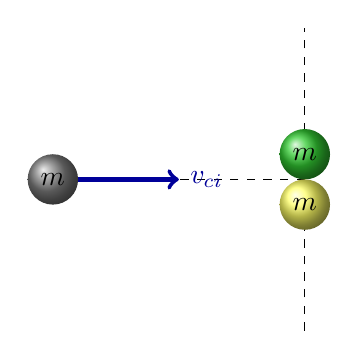
\begin{tikzpicture}[scale=.8]
      \tikzstyle{balloon1}=[ball color=yellow!60];
      \tikzstyle{balloon2}=[ball color=green!60!gray];
      \tikzstyle{balloon3}=[ball color=gray];
      \draw[dashed](0,-2.4)--(0,2.4);
      \draw[dashed](0,0)--(-4,0);
      \shade[balloon2] (0,.4) circle (.4) node{$m$};
      \shade[balloon1] (0,-.4) circle (.4) node{$m$};
      \draw[ultra thick,->,blue!60!black](-4,0)--(-2,0)
      node[pos=1,right]{$\mb{v}_{ci}$};
      \shade[balloon3] (-4,0) circle (.4) node{$m$};
    \end{tikzpicture}
    \hspace{1in}
    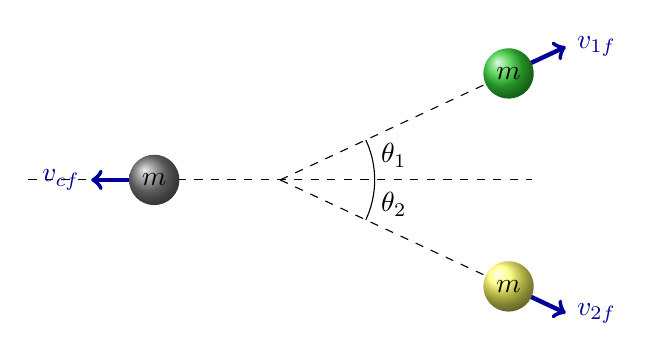
\begin{tikzpicture}[scale=.8]
      \tikzstyle{balloon1}=[ball color=yellow!60];
      \tikzstyle{balloon2}=[ball color=green!60!gray];
      \tikzstyle{balloon3}=[ball color=gray];
      \draw[dashed](-4,0)--(4,0);
      \begin{scope}[rotate=25]
        \draw[dashed](0,0)--(4,0);
        \draw[ultra thick,->,blue!60!black](4,0)--(5,0)
        node[pos=1,right]{$\mb{v}_{1f}$};
        \shade[balloon2] (4,0) circle (.4) node{$m$};
      \end{scope}
      \begin{scope}[rotate=-25]
        \draw[dashed](0,0)--(4,0);
        \draw[ultra thick,->,blue!60!black](4,0)--(5,0)
        node[pos=1,right]{$\mb{v}_{2f}$};
        \shade[balloon1] (4,0) circle (.4) node{$m$};
      \end{scope}
      \draw(1.5,0) arc(0: 25:1.5) node[pos=.6,right]{$\theta_1$};
      \draw(1.5,0) arc(0:-25:1.5) node[pos=.6,right]{$\theta_2$};
      \draw[ultra thick,->,blue!60!black](-2,0)--(-3,0)
      node[pos=1,left]{$\mb{v}_{cf}$};
      \shade[balloon3] (-2,0) circle (.4) node{$m$};
    \end{tikzpicture}
  \end{center}
  \vspace{\stretch{1}}
  
\item A stream of glass beads, each with a mass of \SI{.5}{\gram}, comes out of
  a horizontal tube at $100$ per second. The beads fall a distance of
  \SI{.5}{\metre} to a balance pan and bounce back to their original height as
  shown in the figure below. How much mass must be placed in the other pan of
  the balance to keep the pointer at zero?
  
  \pic{.5}{balance.jpg}
  \vspace{\stretch{1}}
\end{enumerate}
\end{document}
